\documentclass[sigconf]{acmart}

\graphicspath{{../figures/}}

%% Rights management information.  This information is sent to you
%% when you complete the rights form.  These commands have SAMPLE
%% values in them; it is your responsibility as an author to replace
%% the commands and values with those provided to you when you
%% complete the rights form.
\setcopyright{acmcopyright}
\copyrightyear{2018}
\acmYear{2018}
\acmDOI{10.1145/1122445.1122456}

%% These commands are for a PROCEEDINGS abstract or paper.
\acmConference[Woodstock '18]{Woodstock '18: ACM Symposium on Neural
  Gaze Detection}{June 03--05, 2018}{Woodstock, NY}
\acmBooktitle{Woodstock '18: ACM Symposium on Neural Gaze Detection,
  June 03--05, 2018, Woodstock, NY}
\acmPrice{15.00}
\acmISBN{978-1-4503-9999-9/18/06}


%%
%% Submission ID.
%% Use this when submitting an article to a sponsored event. You'll
%% receive a unique submission ID from the organizers
%% of the event, and this ID should be used as the parameter to this command.
%%\acmSubmissionID{123-A56-BU3}

%%
%% The majority of ACM publications use numbered citations and
%% references.  The command \citestyle{authoryear} switches to the
%% "author year" style.
%%
%% If you are preparing content for an event
%% sponsored by ACM SIGGRAPH, you must use the "author year" style of
%% citations and references.
%% Uncommenting
%% the next command will enable that style.
%%\citestyle{acmauthoryear}

\begin{document}

%% The "title" command has an optional parameter,
%% allowing the author to define a "short title" to be used in page headers.
\title[GEODE: Density-Aware Geospatial Query Evaluation on the Edge]{GEODE: Density-Aware Geospatial Query Evaluation \\ in IoT and Edge Environments}

%%
%% The "author" command and its associated commands are used to define
%% the authors and their affiliations.
%% Of note is the shared affiliation of the first two authors, and the
%% "authornote" and "authornotemark" commands
%% used to denote shared contribution to the research.
\author{Ryan Dielhenn, Davin Jimenez, Gabriel Cisneros, and Matthew Malensek}
\affiliation{%
  \institution{Department of Computer Science \\ University of San Francisco}
  %\streetaddress{P.O. Box 1212}
  \city{San Francisco}
  \state{California}
  %\postcode{}
}
\email{{rdielhenn,djjimenez,gcisneros,mmalensek}@usfca.edu}

%%
%% By default, the full list of authors will be used in the page
%% headers. Often, this list is too long, and will overlap
%% other information printed in the page headers. This command allows
%% the author to define a more concise list
%% of authors' names for this purpose.
\renewcommand{\shortauthors}{Trovato and Tobin, et al.}

%%
%% The abstract is a short summary of the work to be presented in the
%% article.
\begin{abstract}
\end{abstract}

%%
%% The code below is generated by the tool at http://dl.acm.org/ccs.cfm.
%% Please copy and paste the code instead of the example below.
%%
\begin{CCSXML}
<ccs2012>
 <concept>
  <concept_id>10010520.10010553.10010562</concept_id>
  <concept_desc>Computer systems organization~Embedded systems</concept_desc>
  <concept_significance>500</concept_significance>
 </concept>
 <concept>
  <concept_id>10010520.10010575.10010755</concept_id>
  <concept_desc>Computer systems organization~Redundancy</concept_desc>
  <concept_significance>300</concept_significance>
 </concept>
 <concept>
  <concept_id>10010520.10010553.10010554</concept_id>
  <concept_desc>Computer systems organization~Robotics</concept_desc>
  <concept_significance>100</concept_significance>
 </concept>
 <concept>
  <concept_id>10003033.10003083.10003095</concept_id>
  <concept_desc>Networks~Network reliability</concept_desc>
  <concept_significance>100</concept_significance>
 </concept>
</ccs2012>
\end{CCSXML}

\ccsdesc[500]{Computer systems organization~Embedded systems}
\ccsdesc[300]{Computer systems organization~Redundancy}
\ccsdesc{Computer systems organization~Robotics}
\ccsdesc[100]{Networks~Network reliability}

%%
%% Keywords. The author(s) should pick words that accurately describe
%% the work being presented. Separate the keywords with commas.
\keywords{datasets, neural networks, gaze detection, text tagging}

%%
%% This command processes the author and affiliation and title
%% information and builds the first part of the formatted document.
\maketitle

%\input{sections/abstract}
\section{Introduction}

As the cost of high-resolution sensors continues to fall alongside steady miniaturization and power efficiency improvements in modern computing hardware, the volume and velocity of observational data streams will continue to grow. In particular, smart cities, self-driving vehicles, smart grids, location-based services, and other types of autonomous systems will rely on real time data streams to make intelligent and timely decisions. These streams often contain readings for several dimensions or \emph{features} and include a spatial component, which may be relative (e.g., SLAM \cite{}) or have specific geospatial coordinates to describe \emph{where} the data was collected.

\textsc{GEODE}: Geopresence Evaluation Over Distributed Edge computing devices.



\section{Related Work}


Galileo \cite{malensek2013polygon,malensek2014evaluating,malensek2016autonomous} supports bitmap-based geospatial queries through its \emph{Geoavailability Grid} data structure. The system allows querying over arbitrary polygons and performs geospatial partitioning for distributed evaluation.  However, the approach does not consider the density of spatial point data; in other words, the Geoavailability Grid hosting data for New York (high density) will have the same resolution as the grid that manages data for Wyoming (low density). Additionally, the approach is stateless and does not support efficient continuous refinement of queries (either through changes to the viewport or polygon of interest), or have a well-defined storage format for fast serialization of matching data points.

. rtrees are bad because they will explode the number of subtrees and lookups will start to take a long time. Look at the book for more weaknesses
. quadtrees don't fan out much so can get even huger than r-trees for big data. 
. From the old CiSE paper: P2PR-Tree \cite{} is a P2P-based version of the R-Tree spatial index. The system is decentralized and can also service
spatial queries while peers are leaving or joining the network. In P2PR-Tree, queries are routed to nodes that may
have pertinent information, with a traversal through the network closely resembling a traversal through an RTree. This traversal pattern allows the system to cope with frequently added or removed nodes, but also involves
additional routing steps that could increase latencies. Initially, the range of possible spatial values is broken up
into blocks, with each block being statically divided into a pre-set number of groups. Nodes in the system are then
divided into multiple levels of subgroups with neighboring peers maintaining more detailed information about one
another. Each peer also maintains a local R-Tree for performing lookups on the data it holds. P2PR-Tree is well-suited for collections of information with geospatial properties, but does not support multidimensional datasets
directly
. maybe beat up on mongo a little bit?

\pagebreak
\section{Index Generation}
% TODO different title? want to make sure this doesn't seem too similar to UCC paper.

Bitmap compression: \cite{antoshenkov1995byte,colantonio2010concise,chan1998bitmap,antoine2011accelerating}

EWAH: \cite{lemire2010sorting}
Roaring: \cite{lemire2016consistently,chambi2016better}

hyperloglog for density

internal geohash MBR

define \emph{station}



%\input{sections/system}
%\pagebreak
\section{Index Generation}
% TODO different title? want to make sure this doesn't seem too similar to UCC paper.

Bitmap compression: \cite{antoshenkov1995byte,colantonio2010concise,chan1998bitmap,antoine2011accelerating}

EWAH: \cite{lemire2010sorting}
Roaring: \cite{lemire2016consistently,chambi2016better}

hyperloglog for density

internal geohash MBR

define \emph{station}



%\section{Retrieval}

splitting the query into separate bitmaps

generating the query bitmap

viewport diffing


%\input{sections/local}
\section{Benchmarks}

We evaluated the performance of GEODE on a 24-node cluster of Raspberry Pi 3 B+ single-board computers (1.4GHz 64-bit quad-core ARMv8 CPU, 1 GB RAM, 
802.11n Wireless LAN, 64 GB microSD storage) running Arch Linux ARM, Kernel 4.19. GEODE C language binaries were produced with all \texttt{gcc} compiler optimizations enabled, and the comparison with Java-based Geoavailability Grids was carried out using OpenJDK 11.0.3.

Notably, the Java VM used for benchmarking had a substantial influence on the results. Our first evaluation of Geoavailability Grids targeted OpenJDK 8, which did not support platform-specific optimizations and ran in a fully-interpreted mode. This yielded run times of over eight minutes for a single iteration of our insertion benchmark. Oracle JDK 8 provides platform-specific optimizations on our test hardware, but its garbage collector is single-threaded by default. Ultimately, we used the latest version of OpenJDK 11 for the benchmarks because parallel garbage collection was supported in addition to platform-specific optimizations.

\subsection{Insertion}

To measure data ingestion performance, we compared the insertion throughput and memory usage of GEODE with the Geoavailability Grid implementation provided in Galileo \cite{malensek2013polygon}. This included the following benchmarks:

\begin{description}
\item[NOAA One Pass:] Inserting a single point for the locations of each station in our NOAA dataset (262,792 unique locations).
\item[NOAA Two Pass:] Repeating the single pass benchmark with a second pass to measure the overhead associated with deserializing messages and converting to index coordinates; the second pass includes the same 262,792 locations and will not cause any changes to the underlying bitmaps.
\item[Random Location:] Entries in observational data streams generally do not exhibit predictable ordering or insertion sequences; this benchmark involved choosing random $(x, y)$ coordinates from a uniform distribution and inserting them into the index.
\end{description}

To establish a baseline performance measure for these benchmarks, additional features beyond the geospatial locations were not stored in memory or on disk.

Figure~\ref{fig:insert} demonstrates insertion throughput, measured by the number of records inserted per second into both index types on a single cluster node. Results were averaged over 100 iterations executed across the entire cluster. Here, GEODE assimilated records approximately 6, 4, and 418 times faster than the Geoavailability Grid implementation.

The speed differential in the NOAA benchmarks can largely be explained by (1) optimizations in converting latitude and longitude to $(x, y)$ grid points, (2) a reduction in the amount of memory allocations performed per insertion, and (3) the Roaring Bitmaps used to manage grid cells are demonstrably faster than the EWAH-based bitmaps in Geoavailability Grids \cite{lemire2016consistently}. The randomized benchmark exhibited a much greater performance differential; while the explanations listed previously for the first two benchmarks do contribute to this disparity, the most significant difference in the two approaches is their underlying bitmap implementations. The Roaring Bitmap-based grids in GEODE allow random insertions, while the EWAH-based bitmaps in Geoavailability Grids require in-order insertions. To compensate for this, random insertions into GeoGrids are batched in a sorted map and flushed periodically, resulting in memory usage fluctuations and higher allocation overhead.

\begin{figure}
    \centerline{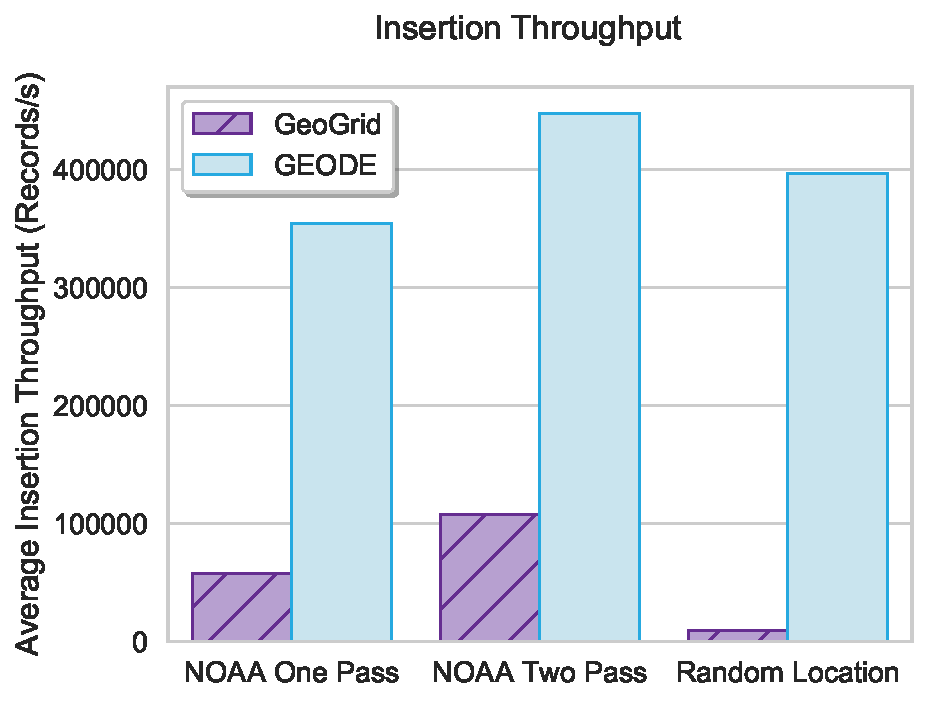
\includegraphics[width=\linewidth]{insert.pdf}}
    \caption{Insertion throughput of GEODE and Geoavailability Grids for each benchmark. Here GEODE maintains substantially higher throughputs, particularly in situations where points are inserted in random order.}
    \label{fig:insert}
\end{figure}

\begin{figure}
    \centerline{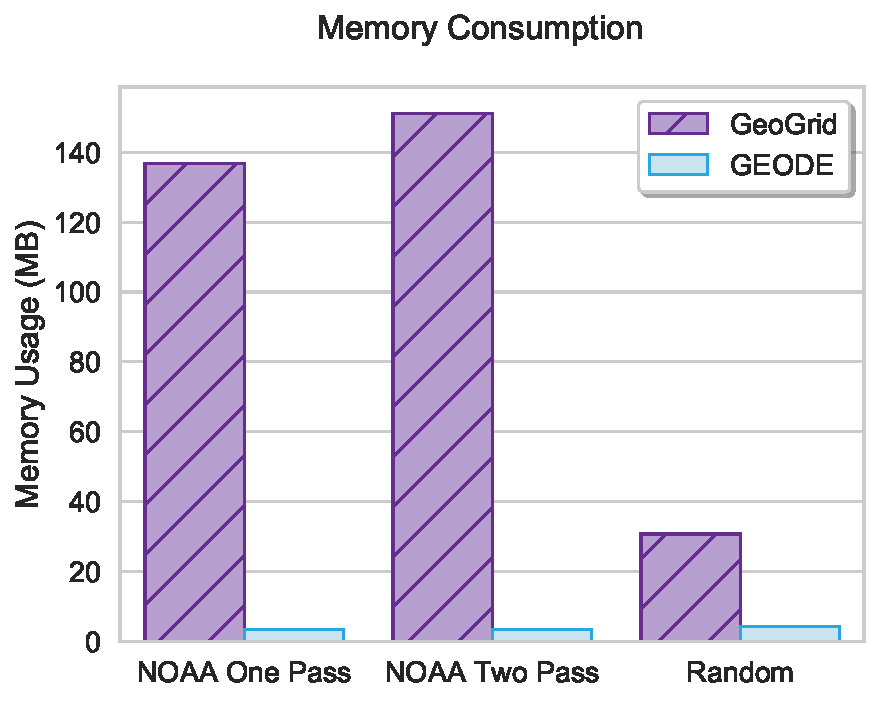
\includegraphics[width=\linewidth]{mem.pdf}}
    \caption{Memory consumed by GEODE and Geoavailability Grids for each benchmark. GEODE requires a more consistent amount of memory and fewer overall allocations.}
    \label{fig:mem}
\end{figure}

\subsection{Querying}

To measure query performance, we compared the query time of GEODE with the Geoavailability Grid implementation provided in Galileo \cite{malensek2013polygon}. This included the following benchmarks:

\begin{description}
\item[Random Location:] Entries in observational data streams generally do not exhibit predictable ordering or insertion sequences; this benchmark involved choosing random $(x, y)$ coordinates from a uniform distribution and inserting them into the index. The index was then queried with a polygon that only spans one geohash so that only one bitmap intersection is performed.
\end{description}

\begin{figure}
    \centerline{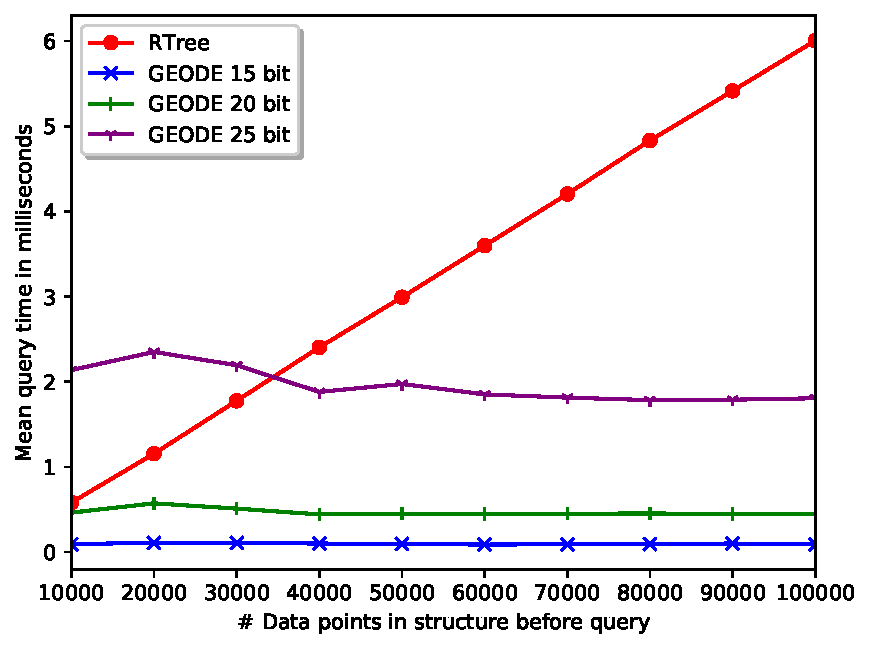
\includegraphics[width=\linewidth]{query_scatter.pdf}}
    \caption{Mean query time of GEODE and Geoavailability Grids after random insertions. GEODE has significantly better query performance compared to the rbang rtree variant, especially with larger data sets. GEODE query time stays consistent regardless of how much data is stored whereas rtree query time increases as data increases. Bitmap resolution does affect GEODE query time, but high resolution bitmaps still beat rtrees with larger datasets.}
    \label{fig:mem}
\end{figure}

%\input{sections/conclusions}
%\input{sections/acknowledgments}

\bibliographystyle{ACM-Reference-Format}
\bibliography{references}

\end{document}
\endinput
